\section{Ejercicio 7}

\subsection{Introducci\'on}
\noindent
En la presente sección se desarrolla la implementaci\'on de dos contadores de 3 bits, uno sincr\'onico y otro asincr\'onico. Se analizan diferencias de funcionamiento entre ambos y se cuantifica la m\'axima velocidad de operaci\'on de cada uno. 

\subsection{Diseño}
\noindent
A continuaci\'on se explican los circuitos utilizados para cada implementaci\'on.

\subsubsection{Contador asincr\'onico}
\label{ej7_sec:cont_asinc}
\noindent
Para la implementaci\'on del contador asincr\'onico se parte del circuito de la Figura 	\ref{ej7_fig:asinc_init}. Tomando N = $Q_2 Q_1 Q_0$, este contador cuenta de 0 a 7 y luego vuelve a comenzar. Se trata de un contador
asincr\'onico porque, como se puede observar, s\'olo el primer Flip-Flop tiene su entrada de CLK conectada a la señal de clock, mientras que los dem\'as se activan con un flanco ascendente de $\overline{Q_{n-1}}$, es decir, un flanco descendente de $Q_{n-1}$. Por lo tanto, tomando como ejemplo el caso de que tenga que activarse el \'ultimo Flip-Flop, a \'este le llega el flanco ascendente luego del retardo de los dos primeros, con lo que no hay sincronismo. \\
%
\begin{figure}[H]
	\centering
	\resizebox{0.7\linewidth}{!}{
			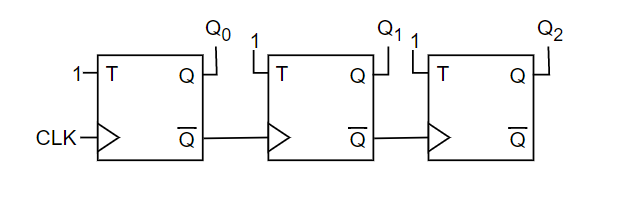
\includegraphics{figs/ej7/ej7_asinc_circ.PNG}	
	}
	\caption{Circuito de un contador asincr\'onico de 3 bits.}
	\label{ej7_fig:asinc_init}
\end{figure}
%
\noindent
Como solamente se dispone de circuitos integrados Flip-Flop D, se utilizan \'estos para obtener los Flip-Flop T que utiliza el circuito. Para ello, se busca una funci\'on l\'ogica que relacione la entrada T y la salida Q con la entrada D que debe tener el integrado para que el circuito se comporte como un Flip-Flop T. La tabla de verdad de dicha funci\'on se muestra en la Tabla \ref{ej7_tab:FFDaFFT}.
%
\begin{table}[H]
\centering
\begin{tabular}{|c|c|c|}
\hline
\textbf{T} & \textbf{Q} & \textbf{D} \\ \hline
0          & 0          & 0          \\ \hline
0          & 1          & 1          \\ \hline
1          & 0          & 1          \\ \hline
1          & 1          & 0          \\ \hline
\end{tabular}
\caption{Tabla de verdad para hacer un FFT a partir de un FFD.}
\label{ej7_tab:FFDaFFT}
\end{table}
%
\noindent
De la tabla de verdad se obtiene que:
%
\begin{equation}
	D = T \oplus Q
\end{equation}
%
Por lo tanto, se obtiene un Flip-Flop T a partir de un Flip-Flop D mediante el circuito de la Figura \ref{ej7_fig:FFDaFFT}.
%
\begin{figure}[H]
	\centering
	\resizebox{0.5\linewidth}{!}{
		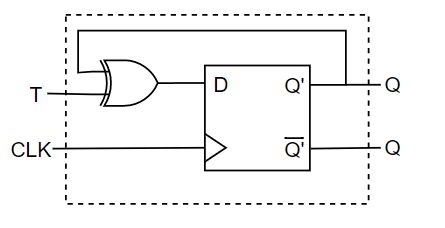
\includegraphics{figs/ej7/ej7_ffd_fft.PNG}
	}
	\caption{Circuito para hacer un FFT a partir de un FFD.}
	\label{ej7_fig:FFDaFFT}
\end{figure}
%
\noindent
Por lo tanto, el circuito definitivo a implementar para el contador sincr\'onico es el de la Figura \ref{ej7_fig:AsincFinal}

%
\begin{figure}[H]
	\centering
	\resizebox{0.9\linewidth}{!}{
		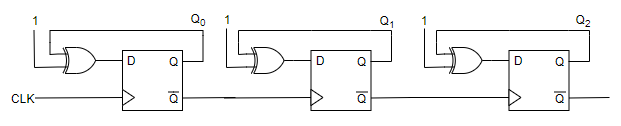
\includegraphics{figs/ej7/ej7_ffd_asinc.PNG}
	}
	\caption{Contador asincr\'onico con FFD.}
	\label{ej7_fig:AsincFinal}
\end{figure}
%
\subsubsection{Contador sincr\'onico}
\noindent
Para el contador asincr\'onico, se parte del contador de la Figura \ref{ej7_fig:sinc_circ}, donde como todos los Flip-Flops est\'an conectados a la señal de clock, se evidencia el sincronismo que le da el nombre a este tipo de contadores. Se trata al igual que en el caso anterior de un contador de 3 bits que cuenta de 0 a 7 y se reinicia. Se incluye en el circuito el bit Z, que vale 1 en el tick anterior a que se reinicie el contador, podr\'ia ser de utilidad dependiendo de la aplicaci\'on.
%
\begin{figure}[H]
	\centering
	\resizebox{0.8\linewidth}{!}{
		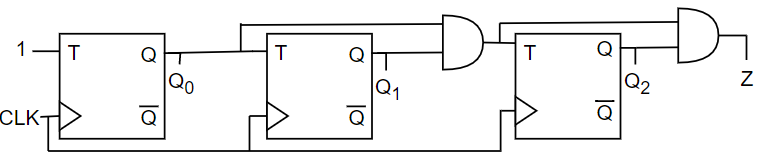
\includegraphics{figs/ej7/ej7_sinc_circ.PNG}
	}
	\caption{Circuito contador sincr\'onico de 3 bits.}
	\label{ej7_fig:sinc_circ_final}
\end{figure}
%
\noindent
Al igual que en la Subsecci\'on \ref{ej7_sec:cont_asinc}, se utilizan Flip-Flops D para realizar las Flip-Flops T, de modo que el circuito definitivo es el de la Figura \ref{ej7_fig:sinc_circ_final}.
%
\begin{figure}[H]
	\centering
	\resizebox{\linewidth}{!}{
		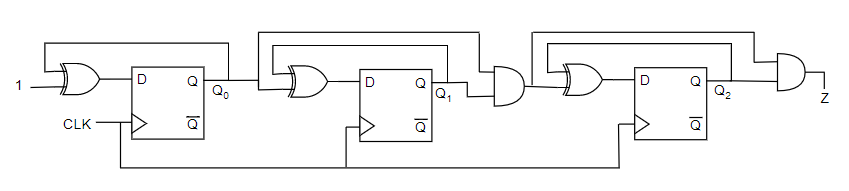
\includegraphics{figs/ej7/ej7_sinc_circ_final.PNG}
	}
	\caption{Circuito del contador sincr\'onico con FFD.}
	\label{ej7_fig:sinc_circ_final}
\end{figure}
%
\subsubsection{Implementaci\'on}
\noindent
Antes de la realizaci\'on se simul\'o el circuito en Proteus para verificar su correcto funcionamiento, en la Figura \ref{ej7_fig:sim_proteus} se muestra la simulaci\'on.
%
\begin{figure}[H]
	\centering
	\resizebox{0.8\linewidth}{!}{
		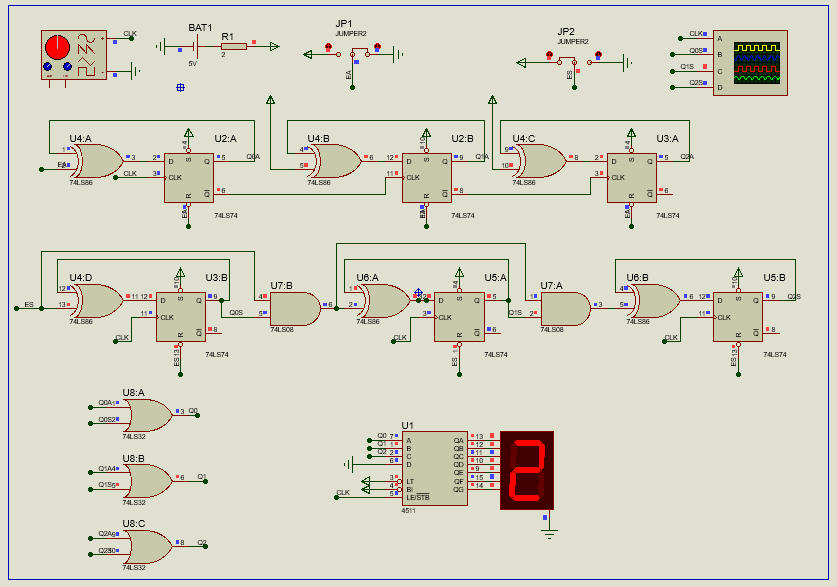
\includegraphics{figs/ej7/ej7_sim_proteus.PNG}
	}
	\caption{Simulaci\'on en Proteus.}
	\label{ej7_fig:sim_proteus}
\end{figure}
%
\noindent
Para la implementaci\'on de los contadores se utilizan compuertas AND, XOR y Flip-Flops D de tecnolog\'ia Low Shottky TTL y se muestra la cuenta en un display LED 7 segmentos. En la Figura \ref{ej7_fig:placa_andando} se muestra una captura de las placas andando.
%
\begin{figure}[H]
	\centering
	\resizebox{0.9\linewidth}{!}{
		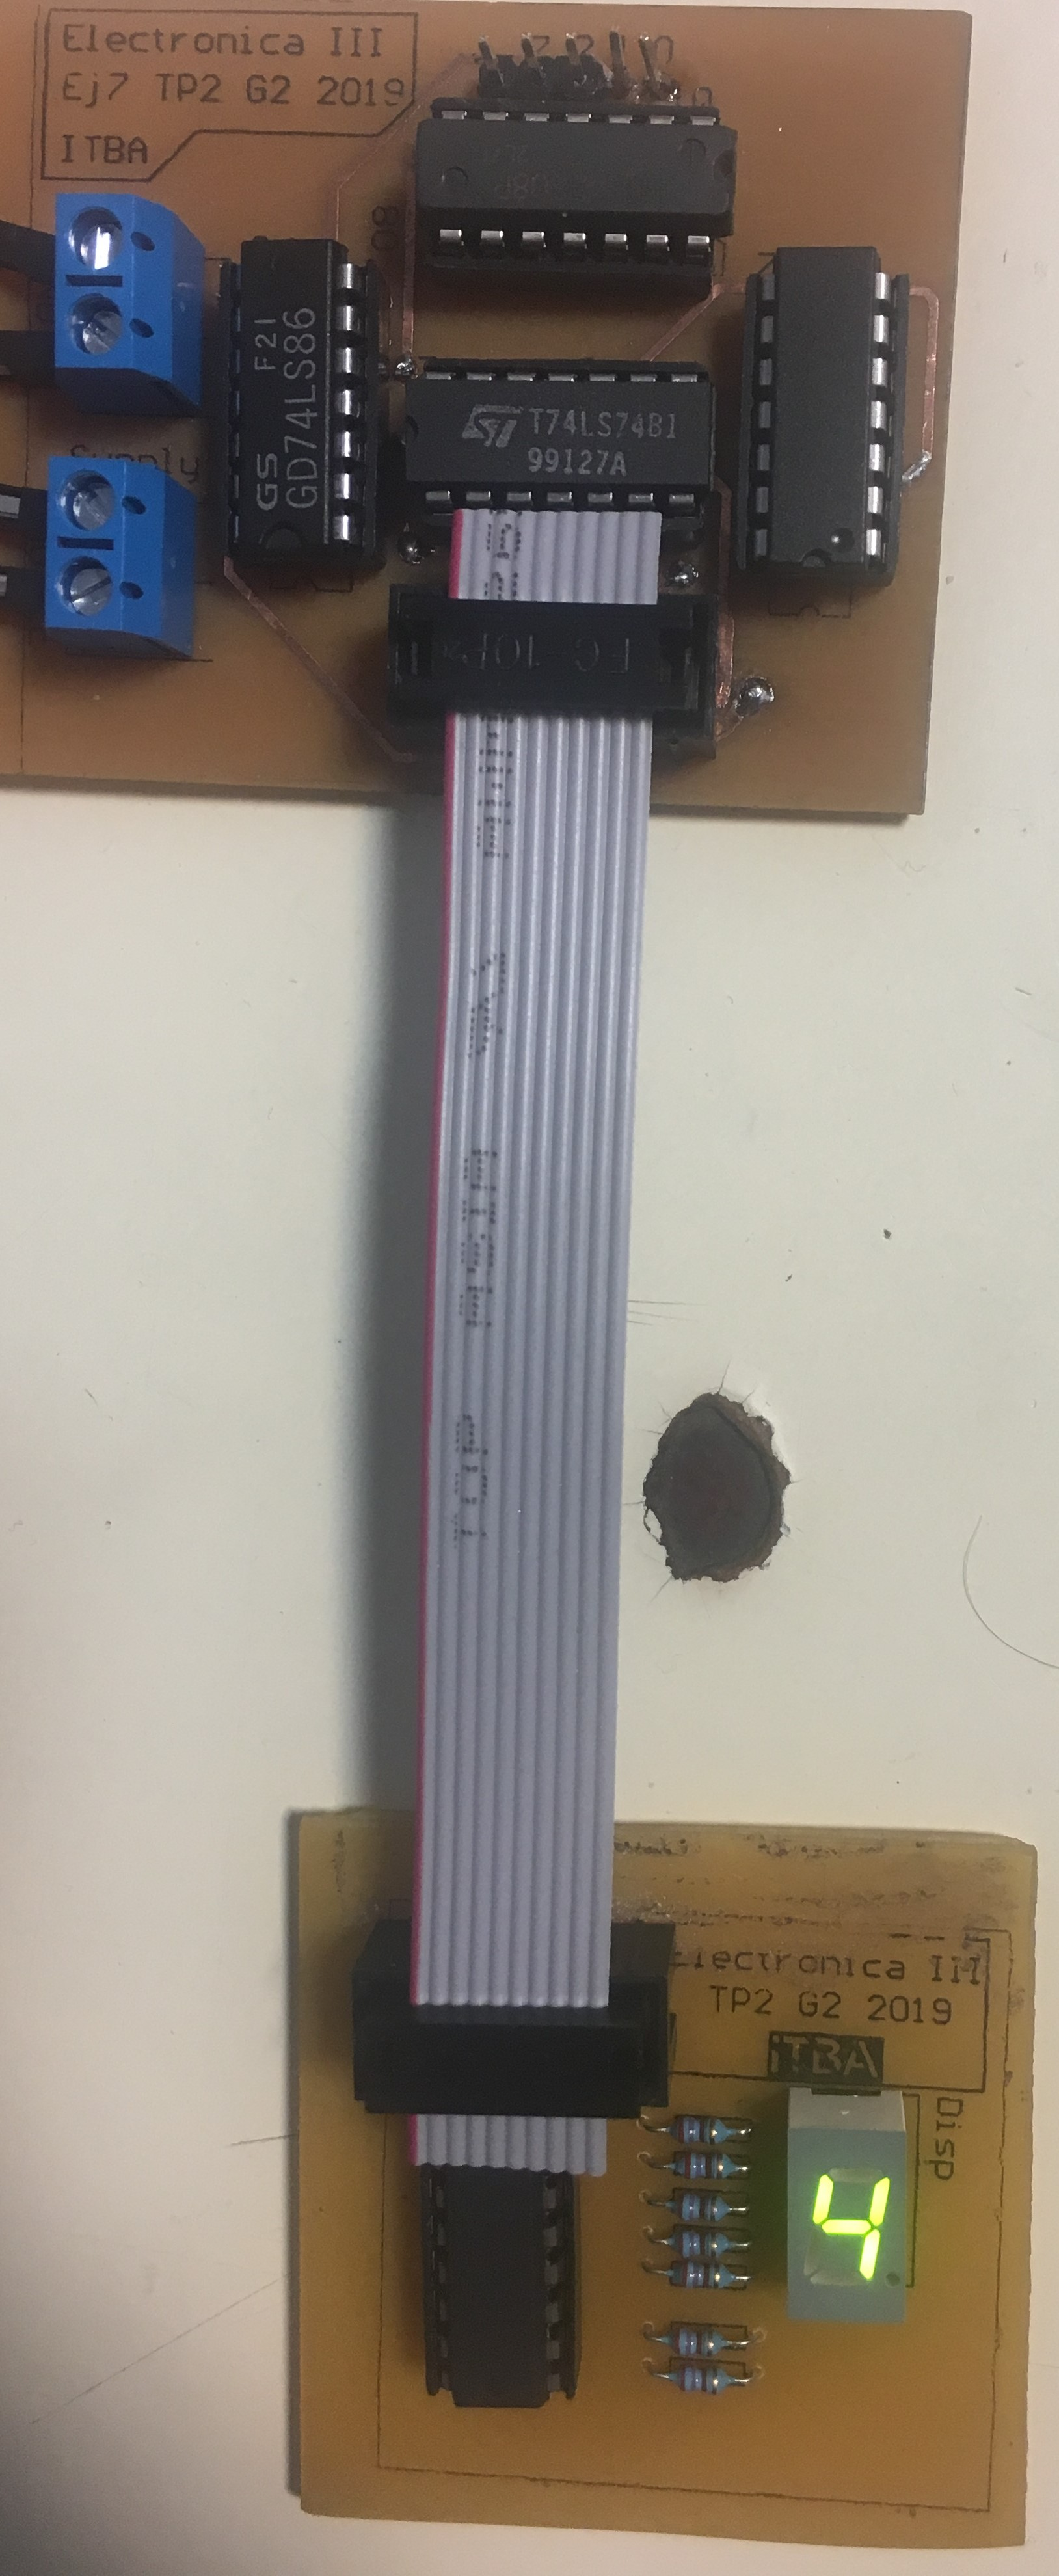
\includegraphics[angle = 90]{figs/ej7/circ_andando.jpeg}
	}
	\caption{Implementaci\'on.}
	\label{ej7_fig:placa_andando}
\end{figure}
%
\subsection{An\'alisis de resultados}
\noindent
A continuaci\'on se muestran las mediciones del funcionamiento de cada contador y sus correspondientes tiempos de propagaci\'on, a partir de los cuales se puede obtener la m\'axima velocidad de operaci\'on.
%
\subsection{Contador asincr\'onico}
\label{ej7_sec:meas_cont_asinc}
\noindent
%En la Figura \ref{} se muestra el funcionamiento del contador asincr\'onico,
En el caso del contador asincr\'onico, se mide el tiempo entre los flancos ascendentes del clock y la respuesta de la señal $Q_2$, que por acarrear los retardos de los otros dos Flip-Flops, es el que mayor retardo presenta. \'Esto se puede comprobar en la Figura \ref{ej7_fig:asinc_0vs2}, donde se observan la señal de clock, los bits $Q_0$ y $Q_2$, y se puede apreciar c\'omo \'este \'ultimo presenta un tiempo de propagaci\'on mayor desde el flanco ascendente de la señal de clock.
%
\begin{figure}[H]
	\centering
	\resizebox{0.7\linewidth}{!}{
		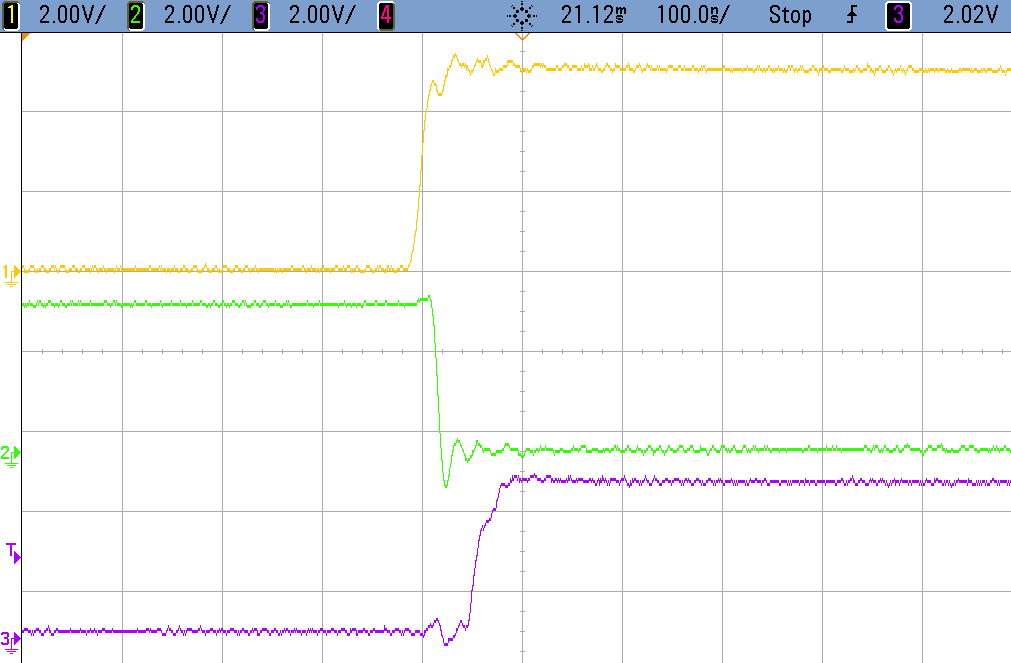
\includegraphics{figs/ej7/cont_asinc_0vs2.png}
	}
	\caption{Clock (amarillo), $Q_0$ (verde) y $Q_2$ (violeta).}
	\label{ej7_fig:asinc_0vs2}
\end{figure}
%
\noindent
Para la medici\'on del tiempo de retardo, se mide el tiempo desde que la señal de clock vale el promedio entre su valor bajo y alto, hasta que la salida toma el valor $V_{OH}$. Para fijar los valores de tensi\'on necesarios para medir, se miden los par\'ametros mencionados del clock, y se busca el valor m\'inimo de $V_{OH}$ en la \href{https://www.ti.com/lit/ds/symlink/sn74s74.pdf}{hoja de datos del fabricante}. Dichos valores se muestran en la Tabla \ref{ej7_tab:valores_medicion}.
%
\begin{table}[H]
\centering
\begin{tabular}{|c|c|}
\hline
\textbf{Par\'ametro} & \textbf{Valor {[}V{]}} \\ \hline
$V_{CLK0}$       & 25m                  \\ \hline
$V_{CLK1}$       & 5,1                    \\ \hline
$V_{CLK50\%}$    & 2,5625                 \\ \hline
$V_{OH}$         & 2,7                    \\ \hline
\end{tabular}
\caption{}
\label{ej7_tab:valores_medicion}
\end{table}
%
\noindent
 Por lo tanto, se mide el tiempo entre que la entrada vale $2,5625V$ hasta que la salida vale $2,7V$. En la Figura \ref{ej7_fig:asinc_measure1} se muestra la medici\'on del tiempo de retardo del bit $Q_2$, de donde se tiene que:
 \begin{equation}
     t_P = 63,3ns
 \end{equation} 
%
\begin{figure}[H]
	\centering
	\resizebox{0.8\linewidth}{!}{
			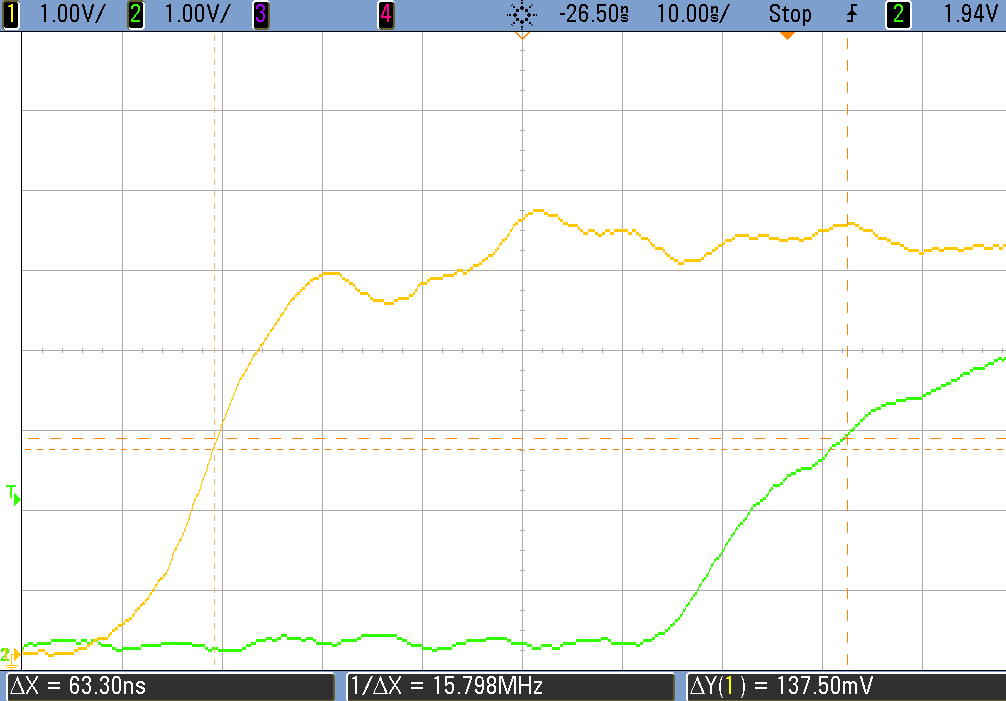
\includegraphics{figs/ej7/cont_asinc_tprop.png}	
	}
	\caption{Medici\'on del tiempo de retardo del contador asincr\'onico.}
	\label{ej7_fig:asinc_measure1}
\end{figure}
%
\noindent
El valor medido est\'a dentro de lo esperado ya los tiempos de propagaci\'on t\'ipicos de los Flip-Flop, $t_{PLH}$ y $t_{PHL}$, son de 14$ns$ y 20$ns$, respectivamente. Teniendo en cuenta que cuando $Q_2$ se activa, $Q_0$ y $Q_1$ pasan al nivel bajo, el tiempo de propagaci\'on del circuito para Flip-Flops t\'ipicos ser\'ia de:
 \begin{equation}
     t_{TIP} = t_{PLH}\cdot 2 t_{PHL} = 74ns
 \end{equation}
 Teniendo el tiempo de propagaci\'on, para determinar la velocidad m\'axima de operaci\'on se pueden tomar distintos criterios. En \'este caso se busca asegurar una velocidad m\'axima para la cual la salida del contador tenga un valor estable en los flancos descendentes de clock, para que al utilizar \'este contador se pueda detectar leer la salida de forma sincr\'onica. Tomando \'este criterio, la m\'axima frecuencia de operaci\'on viene dada por:
 \begin{equation}
     f_{max} = \frac{1}{2\cdot t_{P}} = 7,9MHz
     \label{ej7_eq:vel_max}
 \end{equation}
\subsection{Contador sincr\'onico}
\noindent
En la Figura \ref{ej7_fig:sinc_allbits} se encuentra la señal de clock y los 3 bits del contador para la cuenta de 0 a 7, se muestra qu\'e valor toma la cuenta en cada per\'iodo de la señal de clock.
%
\begin{figure}[H]
	\centering
	\resizebox{0.8\linewidth}{!}{
			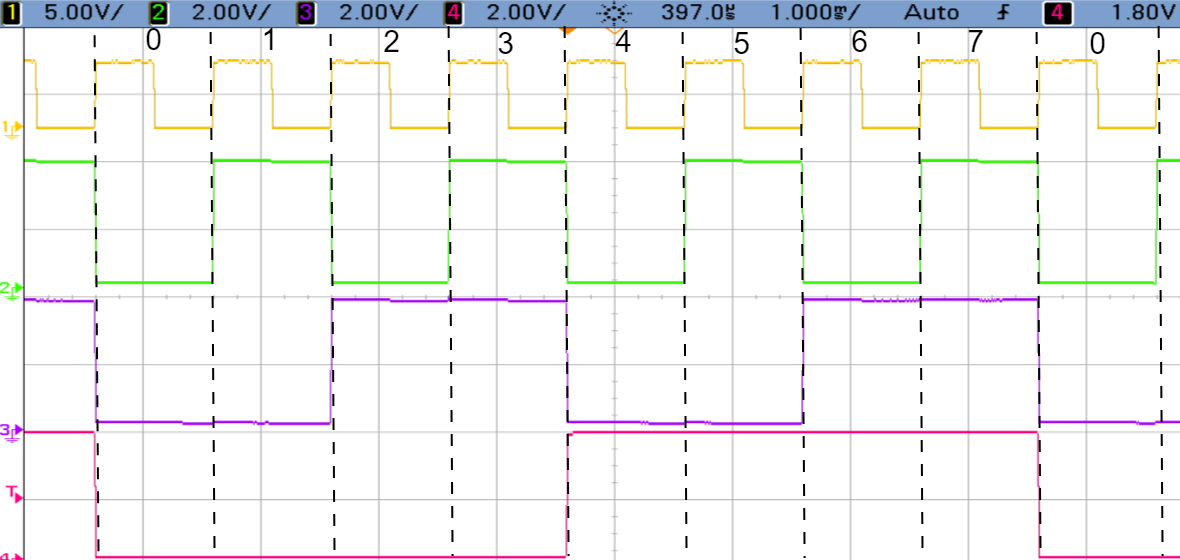
\includegraphics{figs/ej7/cont_sinc_allbits2.png}	
	}
	\caption{Señal de clock (amarillo) y los 3 bits del contador.}
	\label{ej7_fig:sinc_allbits}
\end{figure}
%
\noindent
Para la medici\'on se toman los mismos par\'ametros que en la Subsecci\'on \ref{ej7_sec:meas_cont_asinc}. En la Figura \ref{ej7_fig:sinc_q0_meas} se muestra la medici\'on del tiempo de propagaci\'on del bit $Q_0$, que es de 32,8$ns$. 
%
\begin{figure}[H]
	\centering
	\resizebox{0.8\linewidth}{!}{
			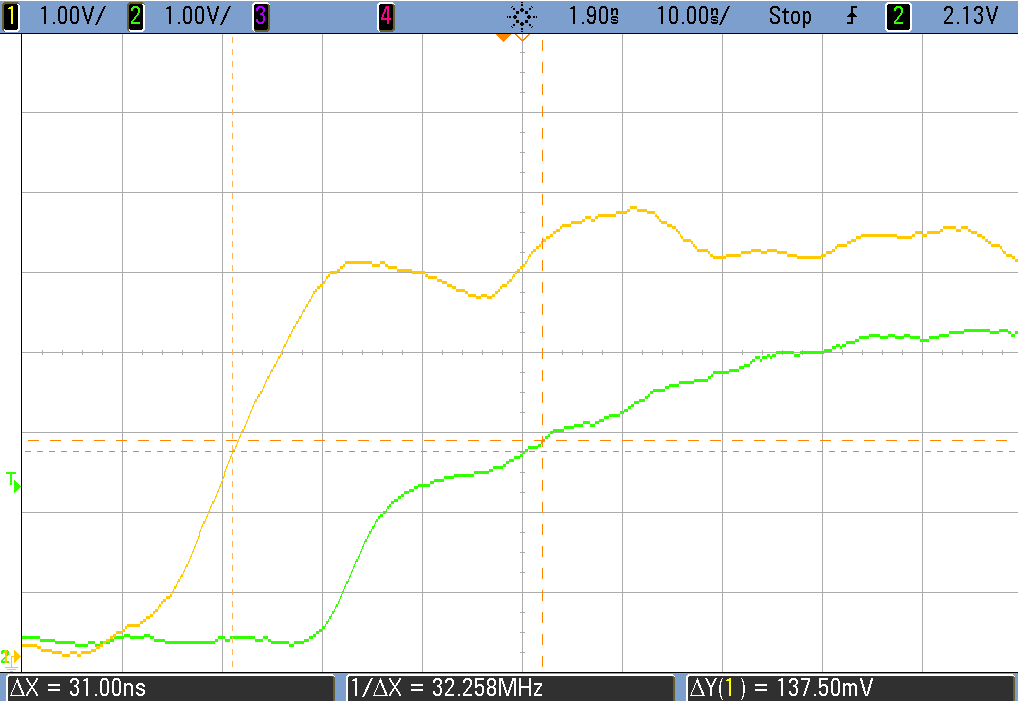
\includegraphics{figs/ej7/cont_sinc_q0_tprop.png}	
	}
	\caption{Medici\'on del tiempo de propagaci\'on del bit $Q_0$ del contador sincr\'onico.}
	\label{ej7_fig:sinc_q0_meas}
\end{figure}
\noindent
Si bien por ser sincr\'onico \'este tiempo deber\'ia ser igual para los 3 bits, se midieron los otros dos bits de la misma forma y se obtuvieron los valores de la Tabla \ref{ej7_tab:t_prop_all}.
%
\begin{table}[H]
\centering
\begin{tabular}{|c|c|}
\hline
\textbf{Bit} & \textbf{$t_p$(ns)} \\ \hline
$Q_0$           & 32,8            \\ \hline
$Q_1$           & 31              \\ \hline
$Q_2$           & 38,1            \\ \hline
\end{tabular}
\caption{Tiempo de propagaci\'on de cada bit del contador sincr\'onico.}
\label{ej7_tab:t_prop_all}
\end{table}
%
\noindent
De los valores medidos, el retardo de $Q_2$ determina la m\'axima velocidad de operaci\'on por ser el mayor. Adoptando el mismo criterio que en el contador asincr\'onico, para la m\'axima velocidad de operaci\'on del contador se obtiene mediante la Ecuaci\'on \ref{ej7_eq:vel_max} que:
\begin{equation*}
    f_{max} = 13,12MHz
\end{equation*}
%
\subsection{Resumen y conclusi\'on}
\noindent
En la siguiente tabla se muestran los valores obtenidos en las mediciones de cada contador.
%
\begin{table}[H]
\centering
\begin{tabular}{|c|c|c|}
\hline
\textbf{Contador} & \textbf{$t_{p}$} & \textbf{$f_{max}$} \\ \hline
Asincr\'onico       & 63,3$ns$           & 7,9$MHz$          \\ \hline
Sincr\'onico        & 38,1$ns$           & 13,12$MHz$        \\ \hline
\end{tabular}
\end{table}
\noindent
Como se esperaba a priori, se observ\'o que el contador sincr\'onico presenta un menor tiempo de propagaci\'on, por lo que en caso de querer trabajar en frecuencias muy altas es importante tener \'esto en cuenta. 